
\typeout{}\typeout{If latex fails to find aiaa-tc, read the README file!}
%


\documentclass[]{aiaa-tc}% insert '[draft]' option to show overfull boxes

\usepackage{mathptmx}         %CHANGE FONT TO TIMES NEW ROMAN

\usepackage{amsmath}          % for formula writing (i.e. 'split', etc)
\usepackage{rotate}           %rotate/mirror images
\usepackage{cancel}           %draw lines through math to show "goes to zero"
\usepackage{xfrac}            %allows slated and side fractions
\usepackage{subcaption}       %allows captioning individual subfigures
\usepackage{multicol}         %enable environment with multiple columns
\usepackage[mode=buildnew]{standalone}% requires -shell-escape
  % compile with `pdflatex -shell-escape main` or `xelatex  -shell-escape main`


\usepackage{tikz}             %for creating vector graphics diagrams
\usetikzlibrary{backgrounds}  %put backgrounds behind tikz figures
\usetikzlibrary{calc}         %perform calculations within $$
\usetikzlibrary{positioning}  %position tikz elements using "right of, etc"
\usetikzlibrary{angles}       %label angles between lines with arcs
\usetikzlibrary{quotes}       %Put angle label in quotes
\usetikzlibrary{patterns}     %Patterns to fill shapes with






  \title{MAE 298 Aeroacoustics -- Final Project \\ Review of Techniques for Predicting Aeroacoustics of Aerospace Vehicles During Launch, Ascent, and Abort}


\author{
  Logan D. Halstrom \\
  {\normalsize\itshape Graduate Student} \\
  {\normalsize\itshape Department of Mechanical and Aerospace Engineering} \\
  {\normalsize\itshape University of California, Davis, CA 95616}
       }


 % Define commands to assure consistent treatment throughout document
 \newcommand{\eqnref}[1]{(\ref{#1})}
 \newcommand{\class}[1]{\texttt{#1}}
 \newcommand{\package}[1]{\texttt{#1}}
 \newcommand{\file}[1]{\texttt{#1}}
 \newcommand{\BibTeX}{\textsc{Bib}\TeX}

%%%%%%%%%%%%%%%%%%%%%%%%%%%%%%%%%%%%%%%%%%%%%%%%%%%%%%%%%%%%%%%%%%%%%%%%
\begin{document}

\maketitle


% % %%%%%%%%%%%%%%%%%%%%%%%%%%%%%%%%%%%%%%%%%%%%%%%%%%%%%%%%%%%%%%%%%%%%%%%%
% \begin{abstract}

% Abstract about lit study

% \end{abstract}





% %%%%%%%%%%%%%%%%%%%%%%%%%%%%%%%%%%%%%%%%%%%%%%%%%%%%%%%%%%%%%%%%%%%%%%%%
% \section*{Nomenclature}

% \begin{multicols}{2}

% \begin{tabbing}
%   XXX \= \kill% this line sets tab stop
%   $0$                 \> Subscript for quiescent parameters \\
%   $e$                 \> Subscript for emission parameters \\
%   $L$                 \> Subscript for loading parameters \\
%   $t$                 \> Time \\
%   $\tau$              \> Retarded time \\
%   $ret$               \> Evaluated at retarded time \\
%   $\hat{n}$           \> Unit surface normal vector \\
%   $\vec{r}$           \> Radial direction vector \\
%   $\hat{r}$           \> Radial unit vector \\
%   $r$                 \> Magnitude of radial vector $|\vec{r}|$ \\
%   $\theta$            \> Angle between $\hat{n}$ and $\hat{r}$ \\
%   $f$                 \> Function of surfaces within a fluid space \\
%   $\vec{V}$           \> General velocity vector \\
%   $V_r$               \> Velocity component in radial direction \\
%   $V_n$               \> Velocity component in surface normal direction \\
%   $M$                 \> Mach number \\
%   $c$                 \> Speed of Sound\\
%   $\overline{\rho}$   \> Mean density \\
%   $p$                 \> Pressure  \\
%   $\widetilde{p}$     \> Pressure (Discontinuous across data surface)  \\
%   $\overline{p}$      \> Mean pressure \\
%   $p'$                \> Perturbation pressure \\
%   $\Delta P$          \> Pressure difference from CFD solution \\
%   $L$                 \> Pressure loading \\
%   $\overline{\partial}$ \> Generalized derivative \\
%   $\delta$            \> Dirac delta function \\
%   \scriptsize{FW-H}   \> Ffowcs Williams-Hawkings\\






% \end{tabbing}

% \end{multicols}




%%%%%%%%%%%%%%%%%%%%%%%%%%%%%%%%%%%%%%%%%%%%%%%%%%%%%%%%%%%%%%%%%%%%%%%%
\section{Introduction} %%%%%%%%%%%%%%%%%%%%%%%%%%%%%%%%%%%%
%%%%%%%%%%%%%%%%%%%%%%%%%%%%%%%%%%%%%%%%%%%%%%%%%%%%%%%%%%%%%%%%%%%%%%%%

Define launch vs ascent vs abort



History of aeroacoustic testing in aerospace vehicles. \cite{SpaceVehicleAeroacousticVibrationPrediction}

analytic modeling for propulsion acoustics.\cite{AcousticPropulsionLoads}




%%%%%%%%%%%%%%%%%%%%%%%%%%%%%%%%%%%%%%%%%%%%%%%%%%%%%%%%%%%%%%%%%%%%%%%%
\section{Experimental Methods}
%%%%%%%%%%%%%%%%%%%%%%%%%%%%%%%%%%%%%%%%%%%%%%%%%%%%%%%%%%%%%%%%%%%%%%%%

One of the most straight forward methods of predicting aeroacoustic vibrational effects on aerospace vehicles is through full-scale testing of sections or complete models of the flight vehicle.  A very detailed summary of design methodologies governing these kinds of test can be found in Himelblau et al. (1970), \cite{SpaceVehicleAeroacousticVibrationPrediction} which will be summarized in the following sections.

The paper specifically addresses the effectiveness of vibrational testing versus acoustic testing of aerospace vehicles.  Vibrational testing facilities utilize electromagnetic or hydraulic shakers to apply vibrational loads to test articles.  Alternatively, acoustic testing involves placing the test article within an acoustic field, similar to that of the flight condition.  At the time of publishing (1970) acoustic testing was relatively new, with its first major usage during the testing of the Titan missile.  Some methods of acoustic testing will now be detailed.


%%%%%%%%%%%%%%%%%%%%%%%%%%%%%%%%%%%%%%%%%%%%%%%%%%%%%%%%%%%%%%%%%%%%%%%%
\subsection{Ground Testing}

The most straight-forward of testing methods described by Himelblau is the free-field test, where the test article is subjected to an outdoor, unconstrained aeroacoustic field produced by some source, an example of which is shown in Fig~\ref{FreeFieldTest}.  The acoustic source in this example is the exhaust of a blowdown wind tunnel, where a fluid upstream of the wind tunnel is pressurized and then released at supersonic speeds through the test section.\cite{BlowdownWindTunnel}  This high pressure fluid then exits the wind tunnel at high speeds, creating conditions similar to that of ascent.



In addition to supersonic wind tunnels, static-fire rocket engine tests can also be used as an acoustic source.  Thus, in the early days of aeroacoustic testing, test could be performed for reduced cost by ``free-riding'' an already existing wind tunnel or rocket engine test.

Acoustic tests can also be performed in more contained facilities.  One example is a reverberant test facility, which is a large chamber surrounded by noise-producing horns.\cite{ReverberantChamber}  These horns allow the production of acoustic vibrations similar to the flight conditions to which sections of the test vehicle can be subjected.

Another method of testing, which was utilized in the ascent certification of the Apollo program lunar and command modules, is the progressive wave facility.  This facility is a chamber with a large number of ducts connecting the test chamber to the outside of the structure, which is excited by an acoustic source (See Fig~\ref{ReverberantTest}).  The ducts are independently operable to allow control of the acoustic conditions inside the test chamber.\cite{ProgressiveWaveChamber}.  This method combines the realistic acoustic source advantages of the free-field test method with some level of source control as found in the reverberant chamber method.





Himelblau demonstrates that these aforementioned acoustic testing methods are superior to traditional vibrational testing methods due to a number of factors:
\begin{enumerate}
  \item Vibration spectra that are more similar to flight conditions
  \item Test article is not constrained at vibration force application points
  \item Ability to test large structural article allows more similar modal characteristics to flight
\end{enumerate}

However, he also states that there are still some limitations when it comes to acoustic testing.  First, it can be difficult to select the proper vibration spectrum for flight condition matching, especially when the acoustic source is a ``free-ride'' wind tunnel or rocket engine test that is not specifically designed for the acoustic experiment.  Additionally, free-field and progressive wave tests may be sufficient in the longitudinal direction parallel to the flow direction, but may not achieve the correct flow characteristics in the circumferential direction perpendicular to the flow.  Finally, the propagation speed of the acoustic test are most likely not identical to that of the flight condition.

For these reasons, it is usually necessary to perform a full-scale flight test as the final certification, which Himelblau details and which is summarized in the next section.

%%%%%%%%%%%%%%%%%%%%%%%%%%%%%%%%%%%%%%%%%%%%%%%%%%%%%%%%%%%%%%%%%%%%%%%%
\subsection{Flight Testing}

A full-scale test flight of an aerospace vehicle is a very expensive operation.  For this reason, Himelblau states that it is highly important to have sufficient instrumentation onboard in order to clearly determine the cause and location of a failure if one occurs.  This is vital in minimizing redesign costs in the case of a failure.

Himelblau reveals that calculations of aeroacoustic effects on structural integrity require a vast amount of data sampling, which was especially constraining in 1970 with limited bandwidth telemetry computers.  For modern tests, the transmission limitation is somewhat alleviated by modern computers, but there is still the additional consideration that many different tests will be running simultaneously during the test flight (e.g. structural, aerodynamic, etc.), and sensor bandwidth must be budgeted between all of these.


%%%%%%%%%%%%%%%%%%%%%%%%%%%%%%%%%%%%%%%%%%%%%%%%%%%%%%%%%%%%%%%%%%%%%%%%
\subsection{Microphone Phased-Array}

A more modern approach to flight test measurements is detailed in the paper by Panda et al. (2013) \cite{MicrophonePhasedArray}, which describes how a microphone phased-array (MPA) can be used to observe launch aeroacoustic conditions accurately from a distance, an example of which is shown in Fig~\ref{MicrophoneArrayPic}.  A MPA is a device that consists of many microphones spread out over some area (e.g. 70 microphones on a 10ft x 10ft area).  The multiplicity of the microphones allows the device to sense not only noise source strength but also location, which is vastly superior functionality to that of traditional single-microphone sensors.

For the test described by Panda, the MPA was designed to maximize lower frequency resolution while adhering to manufacturability constraints.  Microphones were constrained from being to close to one another and also could not occupy the center where a camera was located.  Adhering to these constraints, sensors were placed in logarithmic spirals traveling outward from a center ellipse, and the empty corners were filled in with additional sensors.  The MPA was mounted to a lift about 400 ft away from the rocket, which was raised 40ft in the air and secured by guy wires to prevent motion of the MPA during launch.

During the static fire and actual launch of the Anteres rocket, the MPA was able to determine very specific information about the acoustic sources, greatest of interest being the dominant noise sources.  It was found that during the static fire, the duct exit was the primary noise source, not the duct exit plume as suggested by previous models.  During launch, the dominant source varied with time, starting with the duct exit, but transitioning to the top of the launch pad as the rocket rotated to avoid the service mast.

Specific source information such as the data produced in this experiment can be extremely useful in determining design improvements that will minimize aeroacoustic effects.






%%%%%%%%%%%%%%%%%%%%%%%%%%%%%%%%%%%%%%%%%%%%%%%%%%%%%%%%%%%%%%%%%%%%%%%%
\section{Analytical Methods}
%%%%%%%%%%%%%%%%%%%%%%%%%%%%%%%%%%%%%%%%%%%%%%%%%%%%%%%%%%%%%%%%%%%%%%%%




%%%%%%%%%%%%%%%%%%%%%%%%%%%%%%%%%%%%%%%%%%%%%%%%%%%%%%%%%%%%%%%%%%%%%%%%
\section{Wind Tunnel Testing}
%%%%%%%%%%%%%%%%%%%%%%%%%%%%%%%%%%%%%%%%%%%%%%%%%%%%%%%%%%%%%%%%%%%%%%%%

Aside from full-scale testing, another method for creating flight-like aeroacoustic conditions is through sub-scale wind tunnel testing.  Modern machining techniques (e.g. laser drilling, additive manufacturing, etc.)\cite{SLSAscentWTT} allow production of orders of magnitude higher fidelity models than in the past.  Fine accuracy modeling of vehicle geometry details is extremely important in recovering the specific aeroacoustic environments that are to be expected on the flight vehicle.

To illustrate modern wind tunnel testing methods for aerospace vehicles, we will look at to analyses for NASA's Space Launch System (SLS) rocket.  The first, Herron et al. 2016 \cite{SLSAscentWTT}, concerns ascent aeroacoustics during transonic flight.  The second, Panda et al. 2011 \cite{HeatedHeliumWTT}, simulates the abort condition, where plumes from the abort rocket motors envelope the vehicle structure, creating additional acoustic effects.

%%%%%%%%%%%%%%%%%%%%%%%%%%%%%%%%%%%%%%%%%%%%%%%%%%%%%%%%%%%%%%%%%%%%%%%%
\subsection{Ascent Wind Tunnel Testing}

For ascent testing of SLS, extremely high fidelity 2.5\% and 4\% models of the rocket were manufactured.  The models could be reconfigured to represent various launch configurations.  The extra-fine geometry details of the model can be admired in Fig~\ref{SLSWTT}.

%%%%%%%%%%%%%%%%%%%%%%%%%%%%%%%%%%%%%%%%%%%%%%%%%%%%%%%%%%%%%%%%%%%%%%%%
\subsection{Abort Wind Tunnel Testing}






%%%%%%%%%%%%%%%%%%%%%%%%%%%%%%%%%%%%%%%%%%%%%%%%%%%%%%%%%%%%%%%%%%%%%%%%
\section{Computational Methods}
%%%%%%%%%%%%%%%%%%%%%%%%%%%%%%%%%%%%%%%%%%%%%%%%%%%%%%%%%%%%%%%%%%%%%%%%


%%%%%%%%%%%%%%%%%%%%%%%%%%%%%%%%%%%%%%%%%%%%%%%%%%%%%%%%%%%%%%%%%%%%%%%%
\subsection{Computational Fluid Dynamics}


%%%%%%%%%%%%%%%%%%%%%%%%%%%%%%%%%%%%%%%%%%%%%%%%%%%%%%%%%%%%%%%%%%%%%%%%
\subsection{Computational Aeroacoustic Analysis}






%%%%%%%%%%%%%%%%%%%%%%%%%%%%%%%%%%%%%%%%%%%%%%%%%%%%%%%%%%%%%%%%%%%%%%%%
\section{Conclusions}
%%%%%%%%%%%%%%%%%%%%%%%%%%%%%%%%%%%%%%%%%%%%%%%%%%%%%%%%%%%%%%%%%%%%%%%%















%%%%%%%%%%%%%%%%%%%%%%%%%%%%%%%%%%%%%%%%%%%%%%%%%%%%%%%%%%%%%%%%%%%%%%%%
\begin{thebibliography}{9}% maximum number of references (for label width)
%%%%%%%%%%%%%%%%%%%%%%%%%%%%%%%%%%%%%%%%%%%%%%%%%%%%%%%%%%%%%%%%%%%%%%%%

\bibitem{OverflowOrionAbortGuidelines}
Childs, R. E., Garcia, J. A., Melton, J. E., Rogers, S. E., Shestopalov, A. J., and Vicker, D. J., ``Overflow Simulation Guidelines for Orion Launch
Abort Vehicle Aerodynamic Analyses'', in {\it 29th AIAA Applied Aerodynamics Conference}, Submitted, 2011.

\bibitem{AcousticPropulsionLoads}
Eldred, K. M. and Jones, G. W., Jr., ``Acoustic load generated by the propulsion system'', NASA SP-8072, 1971.

\bibitem{SLSAscentWTT}
Herron, A. J., Crosby, W. A., and Reed, D. K., ``Overview of the Space Launch System Ascent Aeroacoustic Environment Test Program'', in {\it 54th AIAA Aerospace Sciences Meeting}, Submitted, 2016.

\bibitem{ShuttlePayloadBayAcoustics}
Hill, R. E., and Coody, M. C., ``Vibration and Acoustic Environments for Payload/Cargo Integration'', AIAA paper 83-0329, Jan 1983.

\bibitem{SpaceVehicleAeroacousticVibrationPrediction}
Himelblau, H., Fuller, C. M., and Scharton, T. D., ``Assessment of Space Vehicle Aeroacoustic-Vibration Prediction, Design and Testing'', NASA CR-1596, July 1970.

\bibitem{LAVA}
Kiris, C. C., Barad, M. F., Housman, J. A., Sozer, E., Brehm, B., and Moini-Yekta, S.,  ``The LAVA Computational Fluid Dynamics Solver'', in {\it 52nd AIAA Aerospace Sciences Meeting}, Submitted, 2014.

\bibitem{BlowdownWindTunnel}
Lockheed Martin,  ``High Speed Wind Tunnel and Test Systems Design Handbook'', Publication Number AER-EIR-13552-E, 2002.

\bibitem{ReverberantChamber}
Murray, F.M.,  ``Operational Characteristics of a 100,000-Cubic-Foot Acoustic Reverberant Chamber'', {\it The Shock and Vibration Bull.} No. 37, P. 5, Jan. 1968, pp. 13-24.

\bibitem{MicrophonePhasedArray}
Panda, J., Mosher, R. N., and Porter, B. J., ``Identification of Noise Sources During Rocket Engine Test Firings and a Rocket Launch Using a Microphone Phased Array'', NASA TM-2013-216625, Dec 2013.

\bibitem{HeatedHeliumWTT}
Panda, J., James, G. H., Burnside, N. J., Fong, R. K., Fogt, V. A., and Ross, J. C., ``Use of Heated Helium to Measure Surface Pressure Fluctuations on the Launch Abort Vehicle During Abort Motor Firing'', AIAA paper 2011-2901.

\bibitem{OrionAbortPlumesControllability}
Vicker, D. J., Childs, R. E., Rogers, S. E., McMullen, M. S., Garcia, J. A., and Greathouse, J. S.,  ``Effects of the Orion Launch Abort Vehicle Plumes on Aerodynamics and Controllability'', in {\it 51st AIAA Aerospace Sciences Meeting}, Submitted, 2013.

\bibitem{ProgressiveWaveChamber}
Wren, R.J., Dorland, W.D., and Eldred, K.M., ``Concept, Design and Performance of the Spacecraft Acoustic Laboratory'', {\it The Shock and Vibration Bull.} No. 37, P. 5, Jan. 1968, pp. 25-54.




\end{thebibliography}




%%\vspace{-2em}
\begin{figure}[htb]
\begin{center}
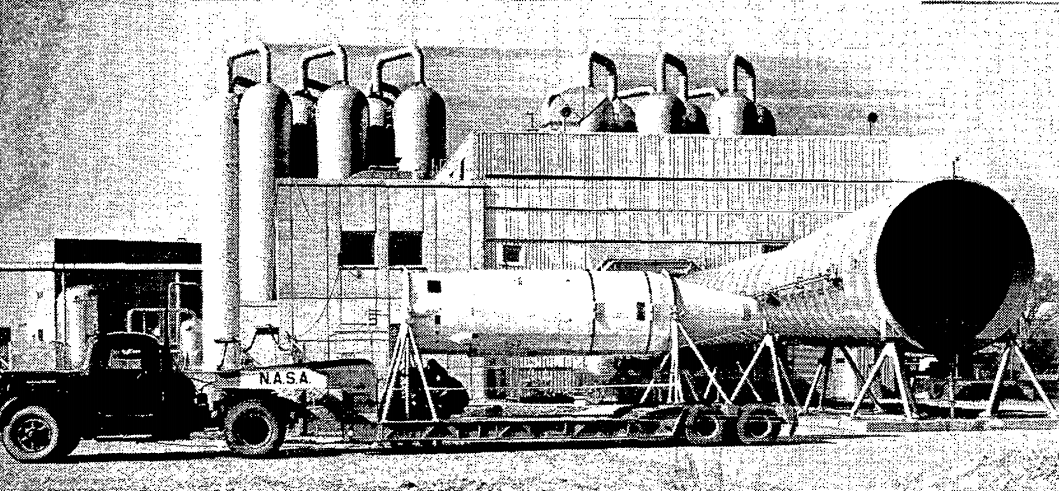
\includegraphics[width=0.7\textwidth]{Images/Himelblau_Fig36.png}
\caption{Acoustic test of the OGO spacecraft near the discharge nozzle of a large blowdown wind tunnel\cite{SpaceVehicleAeroacousticVibrationPrediction}}
\label{FreeFieldTest}
\end{center}
\end{figure}
%%\vspace{-2em}


%%\vspace{-2em}
\begin{figure}[htb]
\begin{center}
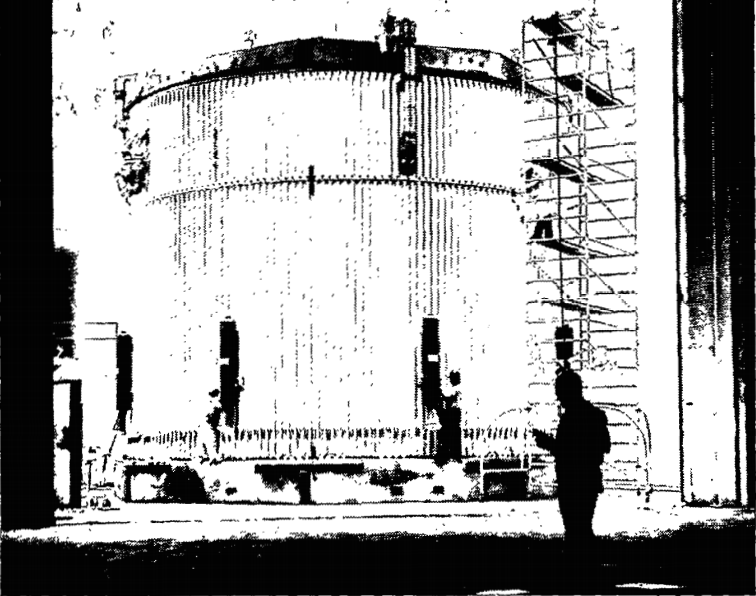
\includegraphics[width=0.7\textwidth]{Images/Himelblau_Fig37.png}
\caption{A Laboratory acoustic test of the thrust structure, aft skirt, and interstage of the S-II stage, Saturn V launch vehicle in a reverberant test facility \cite{SpaceVehicleAeroacousticVibrationPrediction}}
\label{ReverberantTest}
\end{center}
\end{figure}
%%\vspace{-2em}


%%\vspace{-2em}
\begin{figure}[htb]
\begin{center}
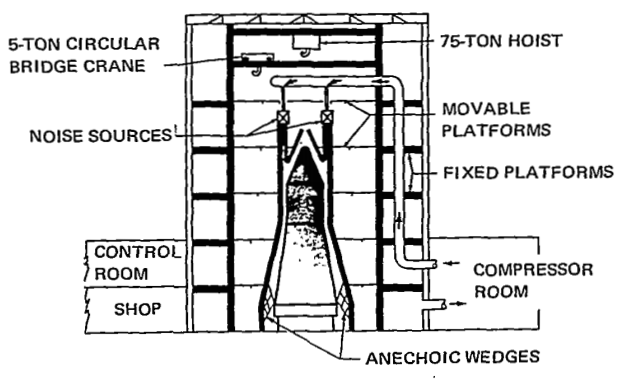
\includegraphics[width=0.7\textwidth]{Images/Himelblau_Fig38.png}
\caption{Laboratory acoustic test of the Apollo spacecraft in a progressive test facility \cite{SpaceVehicleAeroacousticVibrationPrediction}}
\label{ProgressiveTest}
\end{center}
\end{figure}
%%\vspace{-2em}

%%\vspace{-2em}
\begin{figure}[htb]
\begin{center}
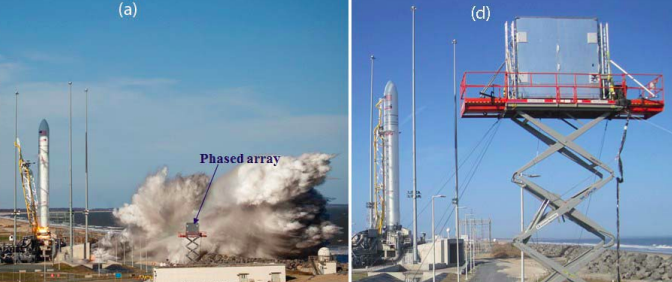
\includegraphics[width=1\textwidth]{Images/MicrophonePhasedArray.png}
\caption{A microphone phased-array observing an Antares rocket launch \cite{MicrophonePhasedArray}}
\label{MicrophoneArrayPic}
\end{center}
\end{figure}
%%\vspace{-2em}

%%\vspace{-2em}
\begin{figure}[htb]
\begin{center}
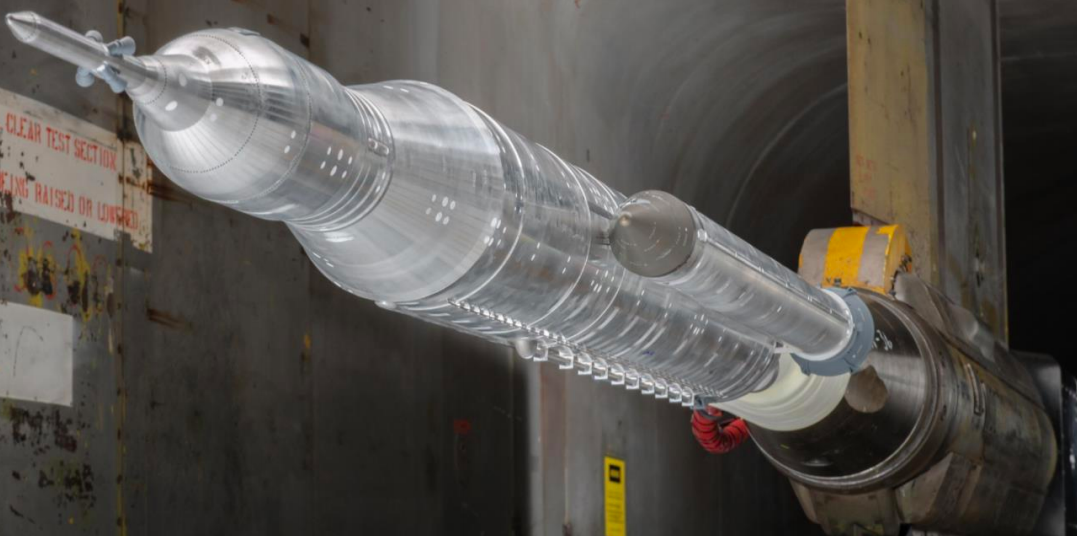
\includegraphics[width=0.95\textwidth]{Images/SLS_WTT_MPCV.png}
\caption{SLS 2.5\% scale wind tunnel model \cite{SLSAscentWTT}}
\label{SLSWTT}
\end{center}
\end{figure}
%%\vspace{-2em}




\end{document}


